\textbf{Problem 2.}

A sequence $\{u_h\}$ converges towards $u$ when $h\rightarrow0$ with order $\alpha$ if there is a finite constant $c$, independent of $h$, such that for sufficiently small $h$
\begin{align*}
    \abs{u_h-u} < ch^\alpha
\end{align*}

\begin{enumerate}[label=(\roman*),leftmargin=*,itemsep=0mm]
    
    \item We wish to determine the order of convergence of the sequence
    $$u_h = \sqrt{h}\sin^2 h$$
    
    Expanding the sequence, we have
    \begin{align*}
        u_h &= \sqrt{h}\sin^2 h
        = h^{1/2} \cdot \left(h-\frac{h^3}{6}\right)^2 \\
        &= h^{5/2} + \mathcal{O}(h^{9/2})
    \end{align*}
    
    Therefore, we see that as $h\rightarrow0$, $u\rightarrow h^{5/2}$ and $\alpha = 9/2$.
    
    \item We wish to determine the order of convergence of the sequence
    $$u_h = \frac{e^h-1-h}{h} = \frac{e^h-1}{h} - 1$$
    
    Expanding the sequence, we have
    \begin{align*}
        u_h &= \frac{e^h-1}{h} - 1
        = \frac{1 + h + h^2/2 + h^3/6 - 1}{h} - 1 \\
        &= \frac{h}{2} + \mathcal{O}(h^2)
    \end{align*}
    
    Therefore, we see that as $h\rightarrow0$, $u\rightarrow h/2$ and $\alpha = 2$.
    
    \item We plot $e_h$ against multiple values of $h$, seeing that $\alpha$ is the gradient (Fig. \ref{hw2_qn2}).  From here, we see that $\alpha = 1$.
    
    \begin{figure*}[h!]
    \centering
    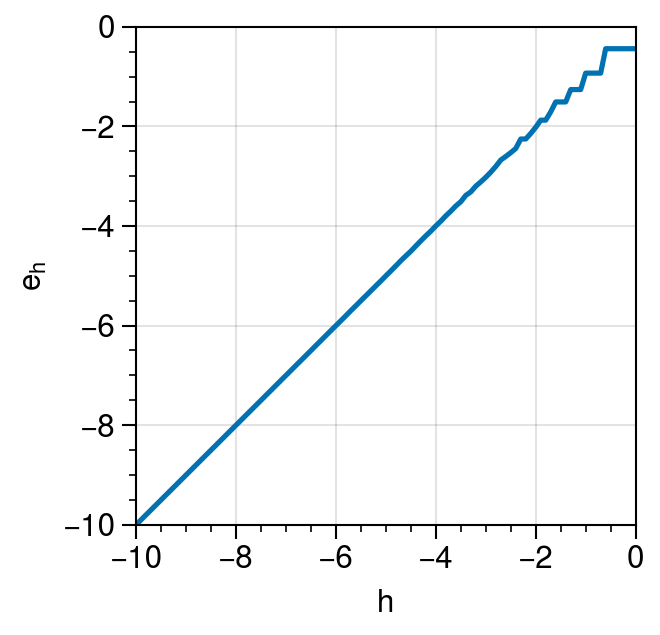
\includegraphics[width=0.2\textwidth]{figures/hw2_qn2.png}\\
    \caption{}
    \label{hw2_qn2}
    \end{figure*}
    
\end{enumerate}